% vqa.tex

\notes{bls better}

% definition
With the goal of optimizing learning computations using quantum computers in
mind, we need an abstract idea of how to implement this connection. A
\emph{Variational Quantum Algorithm} (VQA) is any such system based on a
proposed architecture for a classically controlled quantum computer
\cite{bharti2021noisy}. \autoref{fig:vqaarch} presents the proposed
architecture. The following subsection presents an expanded view of the
computation.

% hybrid diagram
\begin{figure}
    \centering
    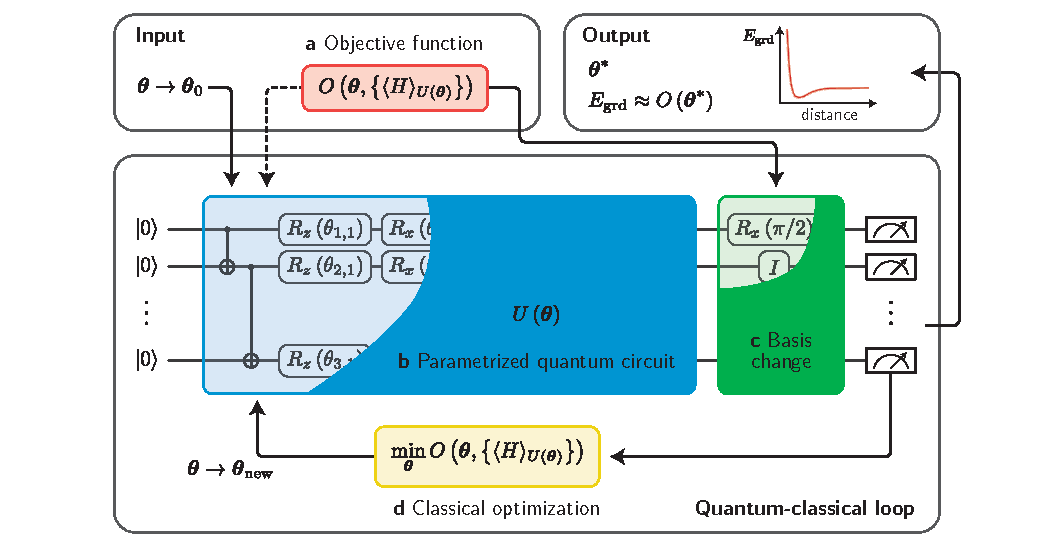
\includegraphics[width=\textwidth]{figures/vqaarch.pdf}
    \caption{Diagrammatic representation of a Variational Quantum Algorithm
    (VQA) \cite[taken from][Figure 2]{bharti2021noisy}.}
    \label{fig:vqaarch}
\end{figure}


\subsection{Building Blocks}

A VQA computation has 4 major components, as shown in \autoref{fig:vqaarch}:

\begin{itemize}
    \item objective function --- the encoding of the problem at hand as an
            optimization,
    \item parametrized quantum circuit (PQC) --- circuit encoding a unitary
            operator parametrized by classically controlled parameters
            \(\vec{\theta}\),
    \item measurement scheme --- the system performing basis changes and
            transferring outputs to the control system, and
    \item classical optimizer --- a classical objective minimizer which controls
            the PQC.
\end{itemize}

These components form a modular computation model where each of the components
can be swapped and improved individually to relieve bottle necks and adapt to the
problem at hand, to control the expressiveness of the system or avoid
treacherous optimization landscapes \cite{larocca2021theory}.

\subsubsection{Objective Function}

The \emph{objective} or \emph{loss function} \cite{larocca2021theory} forms the
target of the optimization problem at hand. This can be any function that can be
encoded in an operational form, i.e., written as or decomposed into quantum
operators. In most cases, this can be expected to be something akin to the
Hamiltonian of a system \cite{bharti2021noisy}, thus making the minimal, ground
state energy, the optimization target. This may also be called the
\emph{parametrized cost} of the computation. Subject to the optimization
constraints, the target of the system is then to find the optimal parameter
input
\begin{gather*}
    % stupid \min isn't working with subcript for some reason
    \parameters_* = \text{arg min}_\parameters\;{\loss(\parameters, p_0(\parameters))}~,
\end{gather*}

where \(p_0(\parameters)\) represents the parametrized probability to measure
the output in the state \(\ket*{0}\).

% pqc
\subsubsection{Parametrized Quantum Circuits (PQCs)}
\label{subsubsec:pqc}
The module central to the design of a VQA is the parametrized quantum circuit,
denoted by \(\pqc(\parameters)\). It is the component of the circuit which
performs the actual `computation' and outputs the state that best meets the
objective. It does so by acting on the input state a series of unitary
transformations parametrized by controllable inputs. We assume the circuit to
have an \(L\)-layered structure as

\begin{gather}
    \pqc(\parameters) = \prod\limits_{l = 1}^{L} U_l(\parameters_l), \quad
    \pqc_l(\parameters) = \prod\limits_{k = 1}^{K} e^{-\iota \theta_{lk} H_k}~,
    \label{eq:pqc}
\end{gather}

where the index \(l\) indicates the layer, and the index \(k\) spans the
traceless Hermitian operators \(\{H_k\}\) that generate the space of unitaries
for the chosen ansatz. Here, \(\parameters\) decomposes as a set of vectors of
parameters \(\vec{\theta}_l\) for each of the indexed layers, which in turn map
to individual parametrized unitary actions indexed by k. Finally, \(M = K \cdot
L\) gives the number of trainable parameters of the system \cite[see][section
II.A]{larocca2021theory}. The experimental apparatus to tune these parameters
depends heavily on the hardware design chosen for the PQC, and may be
mechanical, electronic, or optoelectronic in practice \notes{Cite}.

This general description of a PQC subsumes most ansatzes studied in literature
\cite{larocca2021diagnosing}. These include the hardware-efficient ansatz
\cite{kandala2017hardware}, quantum alternating operator ansatz (QAOA)
\cite{farhi2014quantum}, Hamiltonian variational ansatz
\cite{wecker2015progress}, quantum optimal control ansatz
\cite{choquette2021quantum}, among others \cite{hadfield2019quantum,
zhu2020adaptive, lee2021progress}. These correspond to specific configurations
of layer sizes and choices of the generators. This generic hardware structure
allows us to use the well-formed foundations of landscape theory
(\autoref{subsec:quantlandscape}) to discuss advantages and limitations of VQAs
independent of the specific problem being tackled with them. 

% expressiveness of pqc
The choice of generators is intimately tied to the reachable states of the
system, and the landscape needed to be traversed to get there. This determines
many things about the VQA, including, but not limited to, the problems solvable
within the framework, and the time and hardware constraints required to train
the system. For further detail, see discussion in
\autoref{subsec:quantlandscape}.

Assuming for now that the space spanned by the generators contains our target
unitary, we proceed with the discussion of the computation. After the
application of the PQC, the initial state \(\ket*{\Psi_0}\) is transformed as

\begin{gather}
    \ket*{\Psi(\parameters)} = \pqc(\parameters)\ket*{\Psi_0}~.
\end{gather}

Typically, the input state is chosen to be a zero-valued product state in the
computational basis representation, i.e., \(\ket*{\Psi_0} = \ket*{00\ldots 00} =
\ket*{0}^{\otimes n}\). Other choices of the initial state may be made based on
the problem requirements, possibly even to depend on some variational parameters
itself as \(\ket*{\Psi_0} = P(\phi) \ket*{0}^{\otimes n}\), with \(P(\phi)\) a
parametrized unitary, and \(\phi\) the set of variational parameters. We discuss
these as subjects of study in the future in \autoref{sec:future}.

\subsubsection{Measurement Scheme}
The measurement scheme is chosen to evaluate probabilities and determine the
relevant coefficients using basis changes as necessary. \notes{new material bls}

\subsubsection{Parameter Optimization and Classical Control}

After obtaining the loss function from the measurement and post-processing, a
classical control system may treat it as output from a black box, at which point
the optimizer may be oblivious of the fact the computation is sourced from a
quantum computer, and apply any optimization technique of choice. Based on the
chosen scheme, the controller readjusts the parameters. 

The optimization technique may be a classical one --- gradient based, Hessian
based, etc --- or quantum-aware, taking advantage of the hardware structure, or
to combat specific issues such as quantum noise
\cite{lavrijsen2020classicalopt,stokes2020quantum,
koczor2019quantum,gacon2021simultaneous,haug2021natural}.

\subsection{Quantum Landscape Theory}
\label{subsec:quantlandscape}

\notes{Better intro here}

In \autoref{subsubsec:pqc}, we suggested the problem of the target unitary not
existing in the space reachable in our circuit configuration. In this section,
we elaborate on this issue, and discuss the related problems of studying the
loss landscape, how it emerges, and how it affects the optimization process. We
begin with a review of Quantum Landscape Theory \cite[see][chapter
II.B]{larocca2021theory}.

To study the landscapes, one must first be aware of the spaces each of the
objects relevant to the computation belong to. This is diagrammatically
illustrated in \autoref{fig:qnnspace}. First, the input parameter set
\(\parameters\) is seen as a vector in \(\reals^M\). The PQC then represents an
embedding of \(\reals^M\) into the unitary space of appropriate size
\(d\in\naturals,~ \mathcal{U}(d)\). Its action on the input state is the map
\(\pqc(\parameters): \hilbertspace \to \hilbertspace\). Finally, the measurement
scheme maps the output state to a real-valued loss, which is used by the
optimizer to recompute the parameters. Succinctly, the action of the model
arises from the following transformations

\begin{gather}
    \reals^M \to \mathcal{U}(d) \to \hilbertspace \to \reals~.
    \label{eq:transformations}
\end{gather}

\begin{figure}[!ht]
    % spaces involved in a qnn
    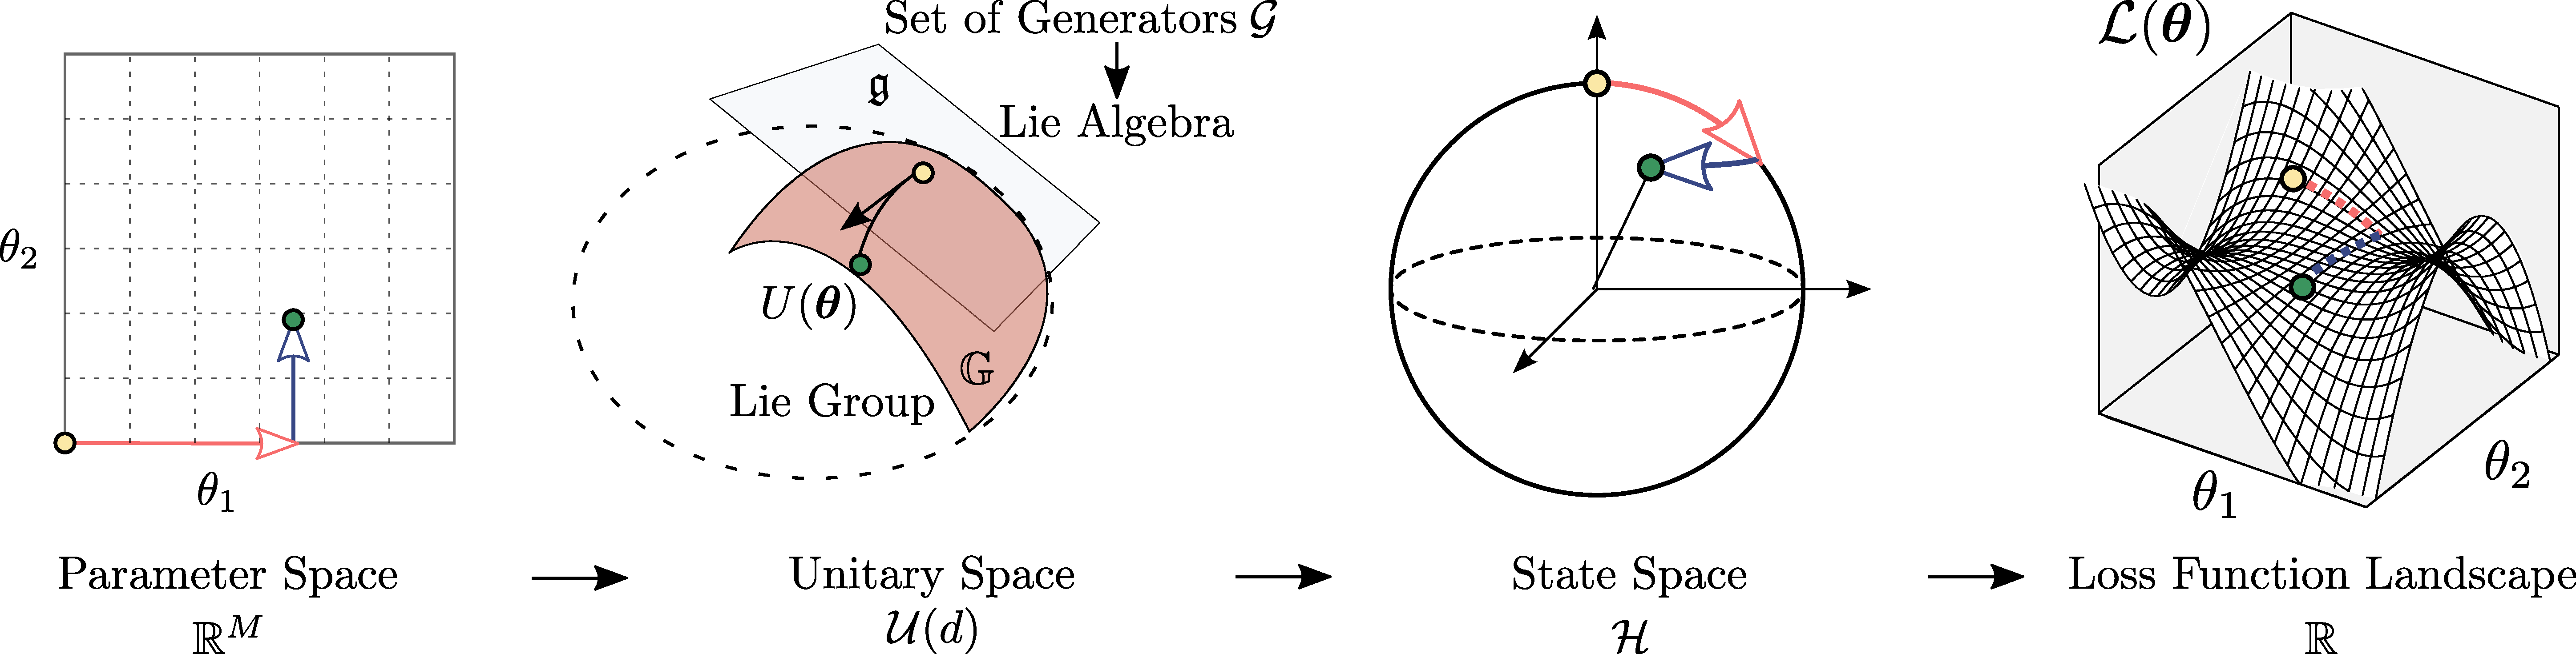
\includegraphics[width=\textwidth]{figures/mapsurjective.pdf}
    \caption{Relevant mathematical spaces for VQA \cite[taken from][Figure
            2]{larocca2021theory}.}
    \label{fig:qnnspace}
\end{figure}

\subsubsection{Parameter Space to Unitary Group \((\reals^M \to
\mathcal{U}(d))\)}

The first map, i.e., the map from the space of parameters to the unitary group,
will be the focal point of the rest of this section. The unitaries generated by
this map, and thus the chosen ansatz, are characterized by an object called the
Dynamical Lie Algebra (DLA) of the system \cite[see][chapter
3]{dalessandro2021introduction}. This represents the space formed by (Lie)
closure of the individual operators in the architecture, under repeated
application and commutation. These operators form the \emph{generators} of the
DLA.

\begin{definition}[Set of Generators]
    Consider a PQC of the form \autoref{eq:pqc}. The set of generators \(\genset
    = \{H_k\}_{k=0}^K\) is defined as the set (of size K) of the Hermitian
    operators that generate the unitaries in a single layer of
    \(\pqc(\parameters)\).
\end{definition}

\begin{definition}[Dynamical Lie Algebra (DLA)]
    Given a set of generators \(\genset\), its DLA \(\dla\) is defined as the
    span of its Lie closure, or the space generated by \(\genset\) after closure
    with repeated nested commutation. Mathematically,

    \begin{equation*}
        \dla = \textup{span } 
        \langle \iota H_1, \iota H_2, \ldots, \iota H_k\rangle_{\text{Lie}}~,
    \end{equation*}

    where \(\langle S \rangle_{\text{Lie}}\) denotes the Lie or the
    nested-commutator closure of \(S\).
\end{definition}

The set of reachable unitaries is then a subset of the Lie group \(\mathbb{G}\)
generated by \(\dla\), 

\begin{equation}
    \{\pqc(\parameters)\}_\parameters \subseteq 
        \mathbb{G} \subseteq \mathcal{SU}(d)~.
\end{equation}

\(\mathbb{G}\) can also be generated completely from the underlying Lie algebra
as \(e^\dla\).

It would seem at first glance that a configuration of generators should be
chosen to be as expressive as possible, which is to have \(\mathbb{G}\) be as
close to \(\mathcal{SU}(d)\) as possible, however, this often leads to
trainability issues such as barren plateaus due to randomly chosen initial
parameters \cite{larocca2021diagnosing,holmes2021connecting,mcclean2018barren}.
As such, the ansatz is generally either chosen to make the problem convenient,
i.e. problem-inspired ansatz \cite{choquette2021quantum}, or to make the
implementation convenient, i.e. hardware-efficient ansatz
\cite{benedetti2021hardware}.

\subsubsection{Unitary Group to State Space \((\mathcal{U}(d) \to
\hilbertspace)\)} 

Recall that for the map from the unitary group to the state space, the unitary
output from the first map acts on states in the input set. Specifically,
choosing the input set to be a training set \(\trainset = \ket*{\psi_\mu}\).
Then, the second map (now parametrized by \(\mu\)) is defined as

\begin{equation}
    \pqc(\parameters) \mapsto \pqc(\parameters)\ket*{\psi_\mu}~.
\end{equation}

The reachable set from each starting state is called its \emph{orbit}. In many
cases, when the states in \(\trainset\) have certain symmetries, the DLA in turn
decomposes as the direct sum of the subspaces invariant under the symmetries

\begin{equation}
    \dla = \bigoplus_\nu \dla_\nu~.
\end{equation}

There is no restriction on whether the states in the training set share or
respect any symmetries of the PQC itself. In this way, the DLA serves as a focal
point to determine the expressiveness in terms of unitaries as well as the set
of reachable states in the Hilbert space.

Next, we wish to see how the output state changes with varying parameters
\(\parameters\). So, consider an infinitesimal perturbation to the parameters
\(\perturbdel \in \reals^M\), and we can then quantify the distance between the
initial and perturbed state. Define \(\ket*{\psi_\mu(\vec{t})} =
\pqc(\vec{t})\ket*{\psi_\mu}\;\forall t \in \reals^m\). Writing the distance
function (second order) as discussed in \autoref{subsubsec:distanceinfo}

\begin{equation}
    d(\ket*{\psi_\mu (\parameters)}, \ket*{\psi_\mu(\parameters + \perturbdel)}) 
        = \frac{1}{2} \perturbdel^\top F_\mu(\parameters) \perturbdel~,
\end{equation}

where \(F_\mu(\parameters)\) is the Quantum Fisher Information Matrix (QFIM) for
\(\ket*{\psi_\mu(\parameters)}\). The QFIM plays a crucial role in quantum-aware
optimizers such as the quantum natural gradient descent
\cite{stokes2020quantum,koczor2019quantum,gacon2021simultaneous,haug2021natural}.
Further, the rank of the QFIM quantifies the number of independent parameters in
the state space that changing the parameters can allow us to explore. The rank
of the QFIM, observed over the whole parameter space, thus gives us a lower
bound on the number of parameters that must be communicated to the PQC to
explore the entire unitary space available to it.

\subsubsection{State Space to Loss Landscape \((\hilbertspace \to \reals)\)}

Finally, the loss landscape generated by the composition map is characterized by
the classically computed landscape of the real-valued loss function, i.e., using
the \(M\times M\) Hessian matrix with indexed entries

\begin{equation}
    \left[\nabla^2 \loss(\parameters) \right]_{ij} = \partial_i\partial_j \loss(\parameters)~.
\end{equation}

Computing the gradient and Hessian matrix allows us to form a quadratic model of
the loss function, with the Hessian's eigenvectors characterizing curvature at
each point. The rank of the Hessian once again gives us the number of
independent directions explorable by change in parameters, emphasizing similarly
how the QFIM functions as a measure of curvature in the state space.
